\documentclass[12pt]{article}
\usepackage{amsmath,amsfonts, epsfig}
\usepackage{booktabs} % for better table formatting
\usepackage{array}
\usepackage{multirow}
\usepackage{graphicx}
\usepackage{fancyhdr}
\usepackage{bm}
\pagestyle{fancy}
\lfoot{\texttt{ematm0067.github.io}}
\lhead{Introduction to AI - 04.2\_pick\_k - Conor}
\rhead{\thepage}
\cfoot{}

\usepackage{tikz}
\usetikzlibrary{positioning}

\usetikzlibrary{shapes.misc}


\usepackage{ifthen,calc}
\newboolean{nopics}
\setboolean{nopics}{false}


\begin{document}

\section*{How to select $k$}

One issue with the $k$-means clustering is how to pick the value of
$k$. Often we are interested in exploring different values, there
might be different clustering structures at different scales, for
example. Sometimes, however, we want to be able to say that the data
shows evidence for some specific number of clusters. Sadly, this rarely works out, or at least, we rarely get a completely satisfactory answer.

We will start out describing how we think it might work. The idea is
to define a measure of the quality of the clusters. If
\begin{equation}
  \mathcal{C}=\{C_1,C_2,\ldots,C_k\}
\end{equation}
is a set of clusters with corresponding centroids $\mathbf{c}_i$ then
one such quantity is
\begin{equation}
  J(\mathcal{C})=\sum_{i=1}^k\sum_{\mathbf{x}_j\in C_i}[d(\mathbf{x}_j,\mathbf{c}_i)]^2=\sum_{i=1}^k\sum_{\mathbf{x}_j\in C_i}|\mathbf{x}_j-\mathbf{c}_i|^2
\end{equation}
This is sometimes called the \textsl{degree of dissimilarity} since it
measures how much the points differ from their centroid. Now it should
be clear that this number goes down as $k$ increases, the question is
what shape that descending curve has. The claim is that there will be
a \textsl{dogs' leg}, a sort of corner where $J(\mathcal{C})$ levels
off suddenly, this means that adding new centroids isn't as useful
anymore and so the dogs' leg corresponds to the best value of $k$.

In Fig.~\ref{fig:points} there are some points with very clear
clusters, it is an artificial dataset intended to have this
structure. In Fig.~\ref{fig:J} the value of $J(\mathcal{C})$ for the
clustering discovered through $k$-means has been plotted. You can see that the fall in the value of $J(\mathcal{C})$ does level out at around five, but, even for this most ideal of datasets, it isn't super obvious''
So, in summary, use $J$ to assess the best value of $k$, but don't be surprised if it isn't super conclusive!




\begin{figure}[htb]
\begin{center}  
  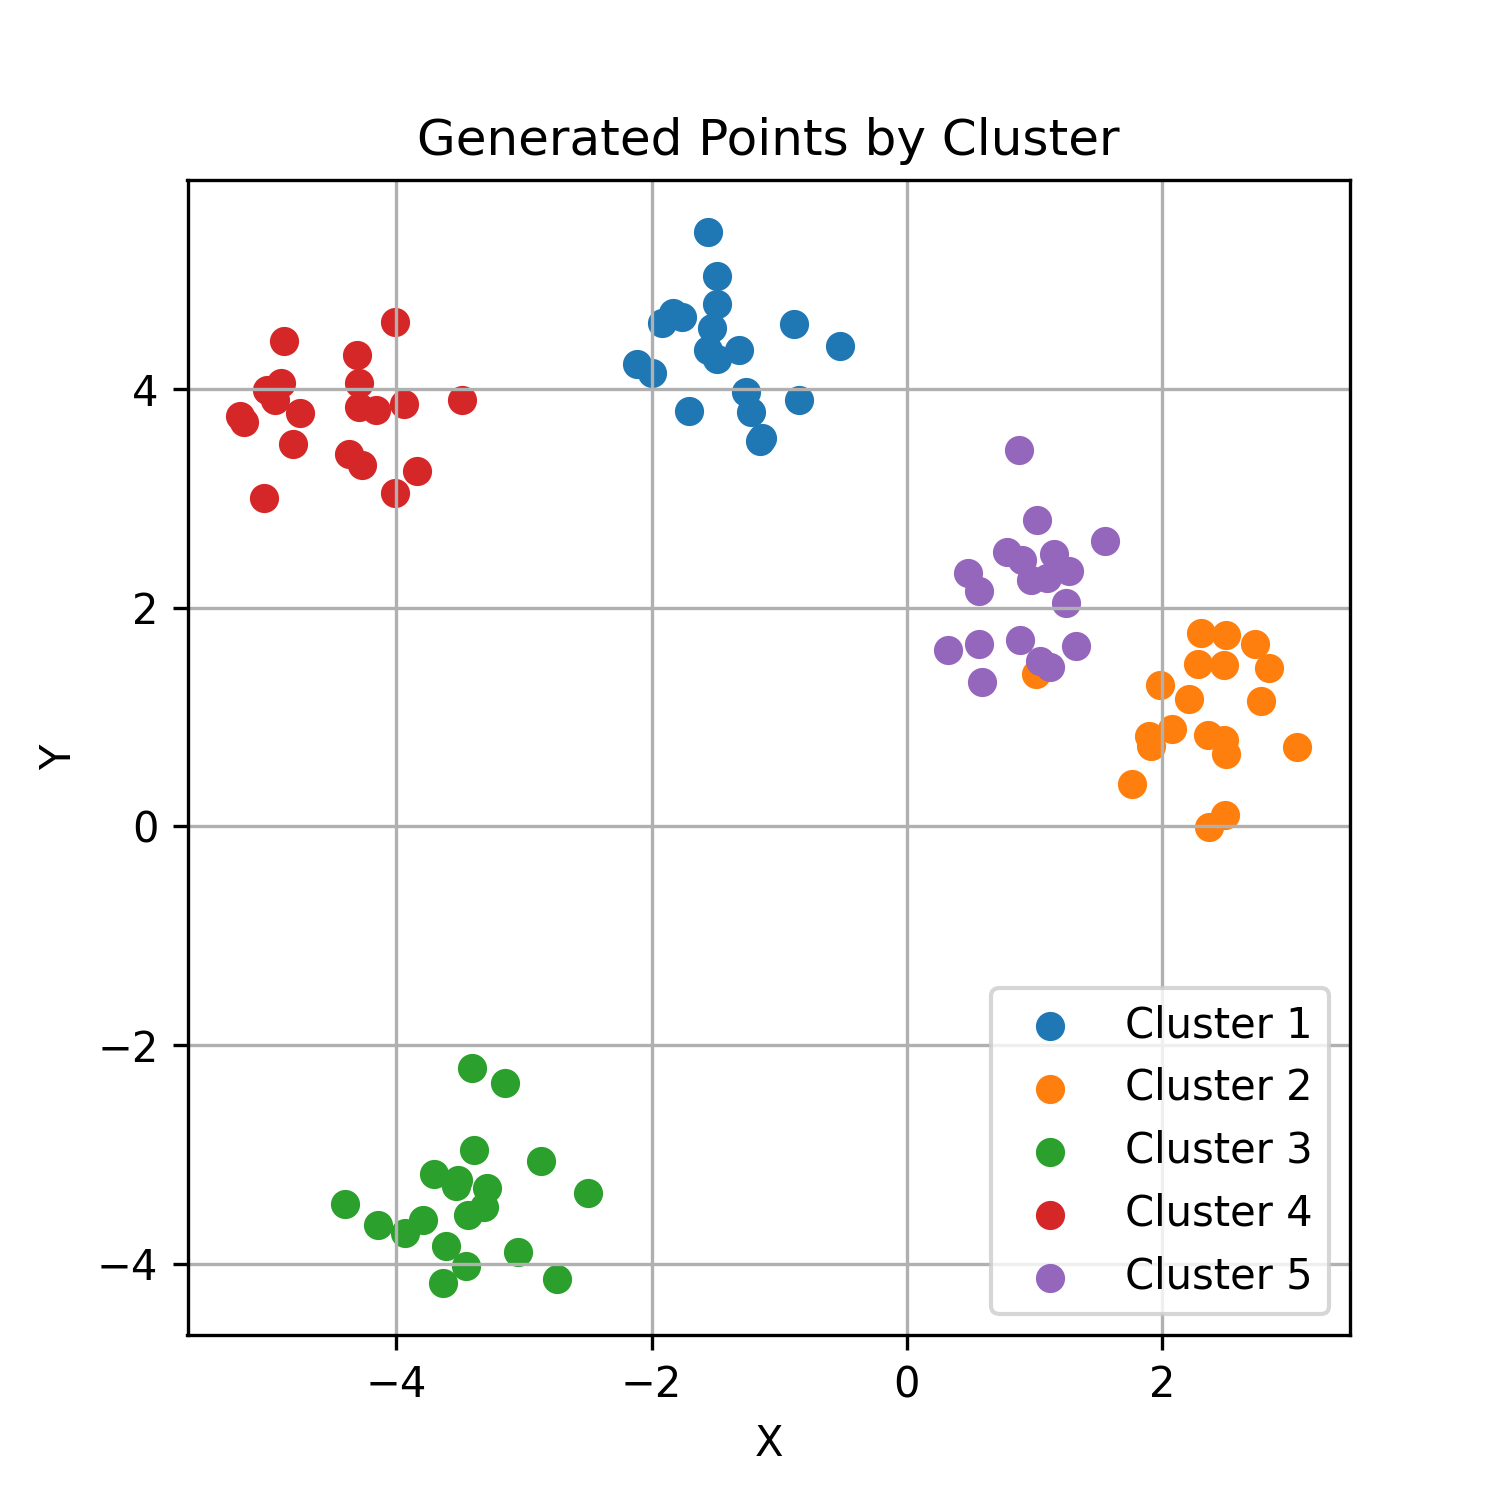
\includegraphics{04.2_points.png}
\end{center}
\caption{In this simulated data set five centers have been picked at random in a ten by ten box, for each center 20 points have been picked using a normal distribution with standard deviation 0.5.\label{fig:points}}
\end{figure}



\begin{figure}[htb]
\begin{center}  
  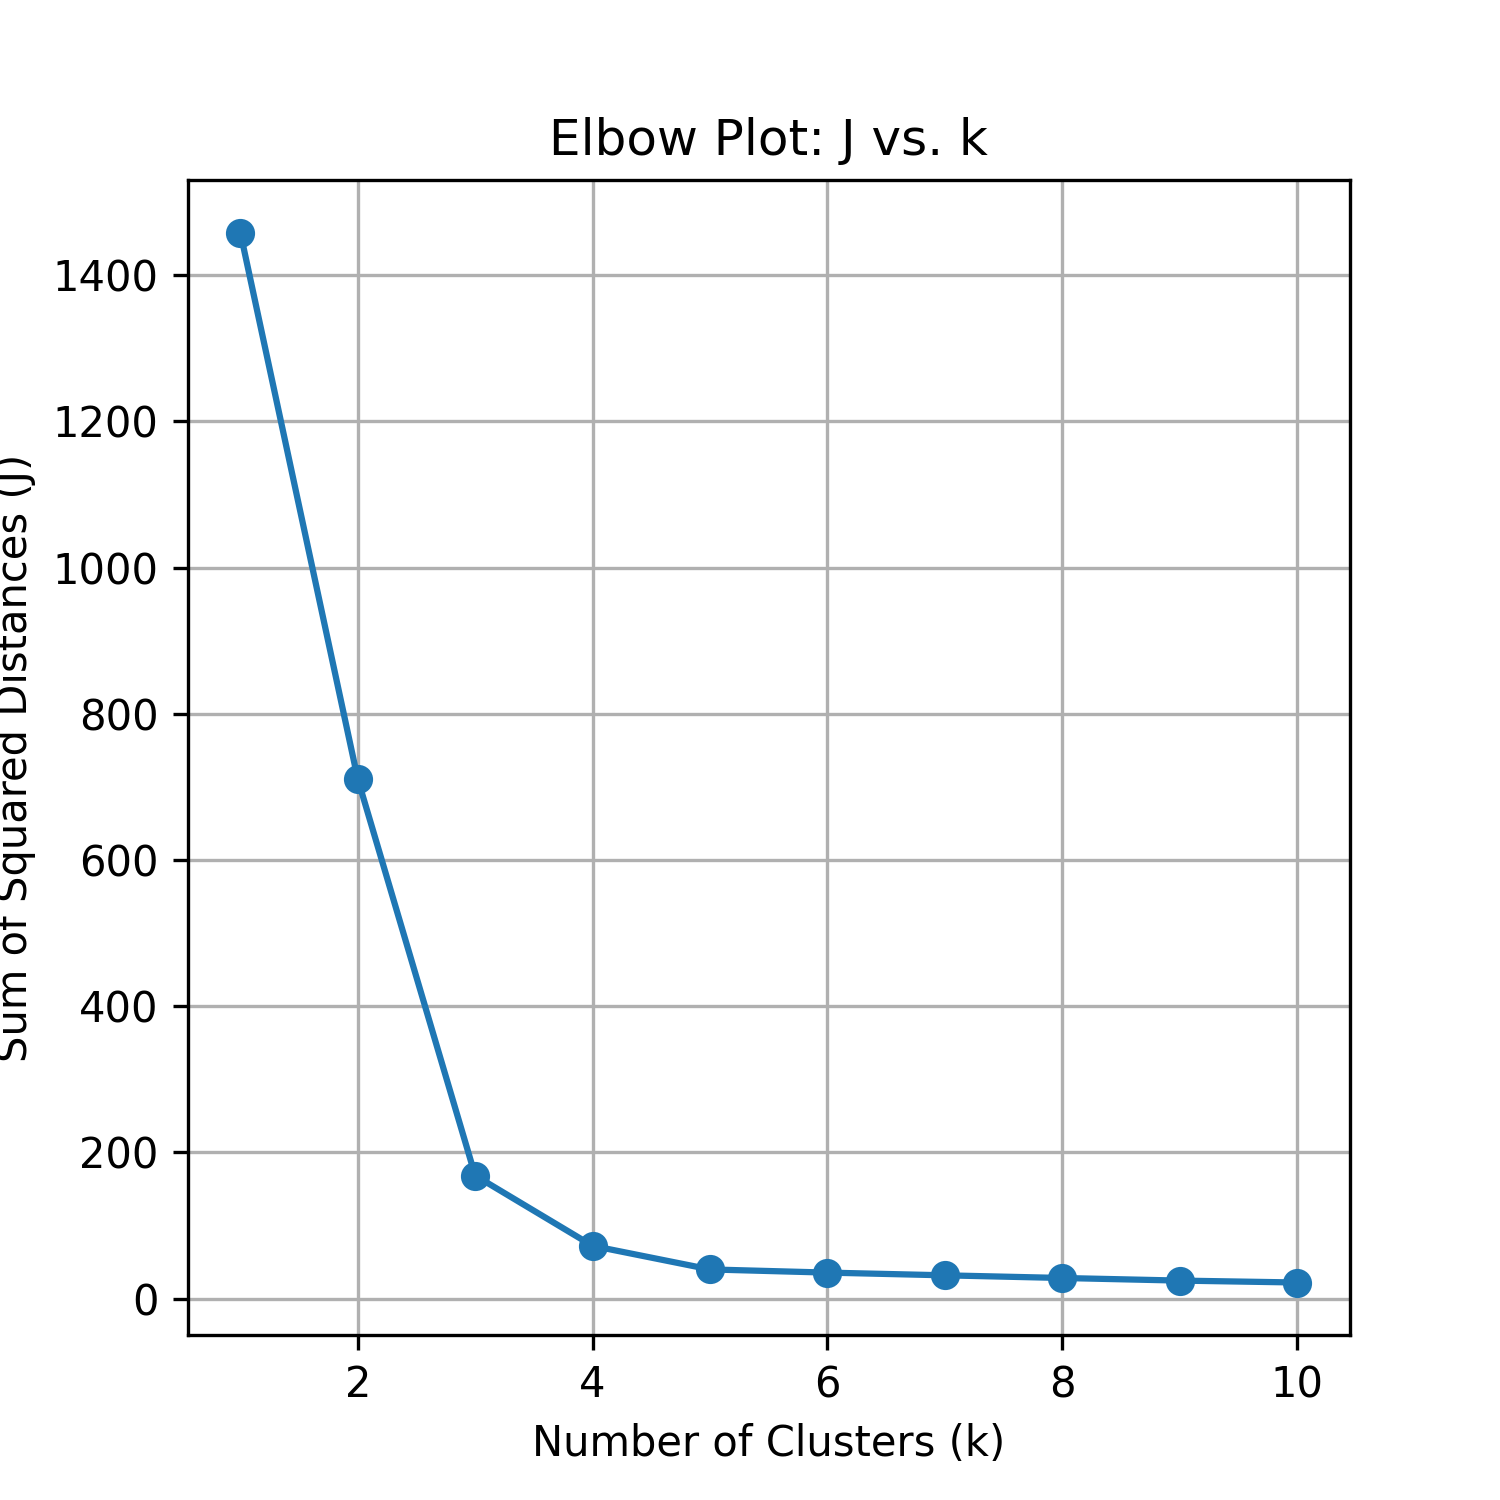
\includegraphics{04.2_J.png}
\end{center}
\caption{For the simulated data the degree of dissimilarity has been
  calculated and is plotted against $k$.\label{fig:J}}
\end{figure}


\end{document}

